\pgfplotsset{compat=1.15}
\setlength{\fboxsep}{0pt}

\begin{tikzpicture}
  \draw
  (0, 8) node[anchor=east]{\small{Input}} to[short, o-]
  ++(1.5, 0) node[anchor=west,inner sep=0](extract){
    \fbox{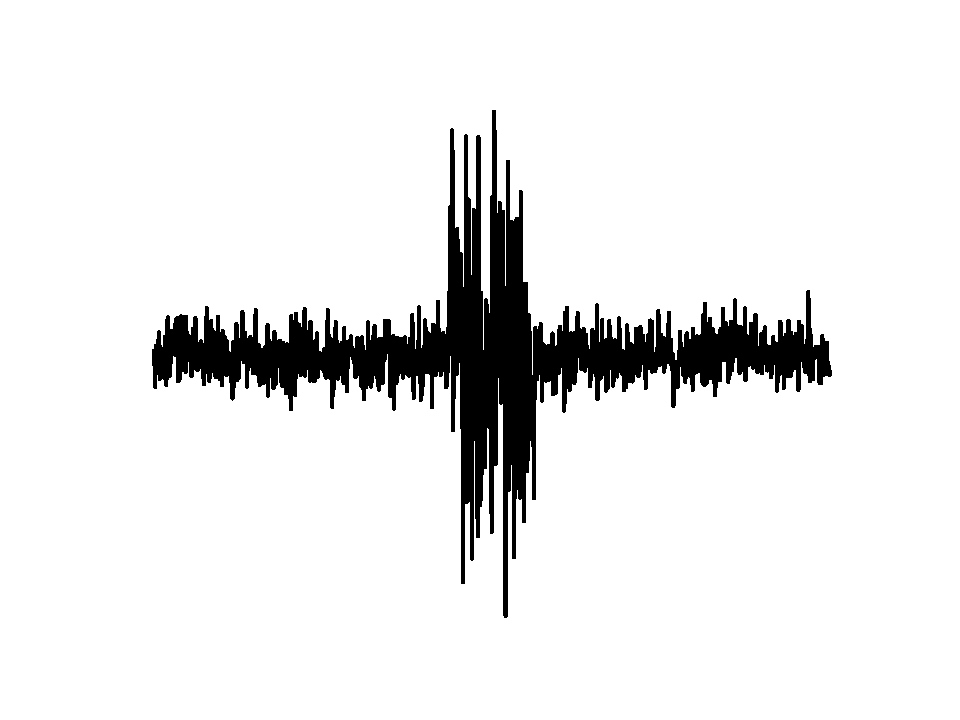
\includegraphics[width=1.5cm]{diagrams/xcorr_tagger_extract.pdf}}
  }
  (extract.east) to[short]
  ++(1.5, 0) to[switch]
  ++(1, 0) to[short]
  ++(1.25, 0) node(move_tag)[minimum width=1.6cm, minimum height=1cm, anchor=west, draw=black, line width=0.25mm, align=center]{\small{Move}\\\small{tag}}
  (move_tag.east) to[short, -o]
  ++(1.5, 0) node[anchor=west]{\small{Output}};

  \draw
  (extract.south) to[short, -*]
  ++(0, -0.4) node[anchor=east, align=center]{\small{Chunk extraction}} to[short]
  ++(0, -0.4) node[anchor=north,inner sep=0](extract_cropped) {
    \fbox{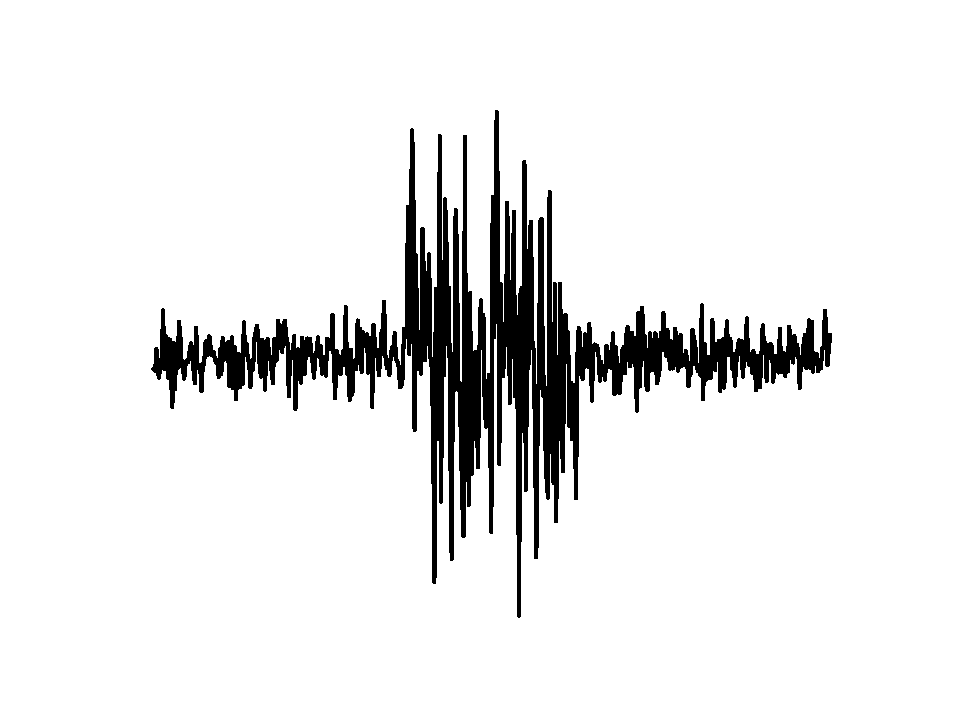
\includegraphics[width=1.5cm]{diagrams/xcorr_tagger_extract_cropped.pdf}}
  }
  (extract_cropped.south) to[short, -*]
  ++(0, -0.4) node[anchor=east, align=center]{\small{Zero padding}} to[short]
  ++(0, -0.4) node[anchor=north,inner sep=0](extract_padded) {
    \fbox{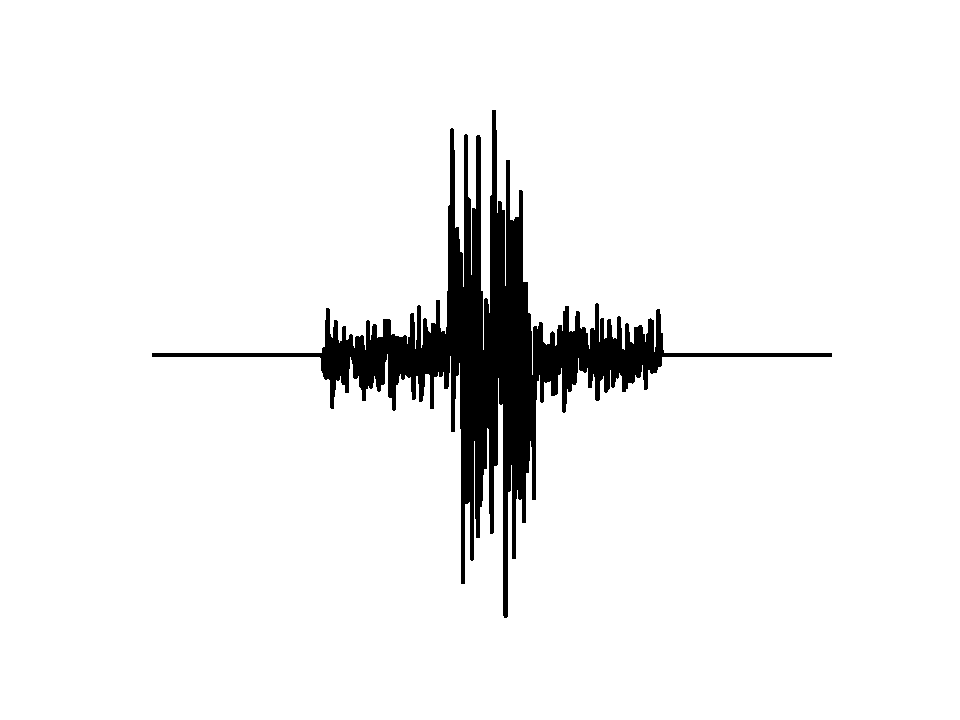
\includegraphics[width=1.5cm]{diagrams/xcorr_tagger_extract_padded.pdf}}
  }
  (extract_padded.south) to[short]
  ++(0, -0.8) node(fft_in)[minimum width=1cm, minimum height=1cm, anchor=north, draw=black, line width=0.25mm, align=center]{FFT}
  (fft_in.east) to[short]
  ++(1.75, 0) node(fft_mul)[mixer, anchor=west]{}
  (fft_mul.east) to[short]
  ++(1.5, 0) node(ifft)[minimum width=1cm, minimum height=1cm, anchor=west, draw=black, line width=0.25mm, align=center]{iFFT};

  \draw
  (fft_in.south)
  ++(0, -1.4) node(fft_ref)[minimum width=1cm, minimum height=1cm, anchor=north, draw=black, line width=0.25mm, align=center]{FFT}
  (fft_ref.east) to[short]
  ++(1.75,0) node(ref_conj)[minimum width=1cm, minimum height=1cm, anchor=west, draw=black, line width=0.25mm, align=center]{$z^\ast$}
  (ref_conj.north) to[short]
  (fft_mul.south)
  (fft_ref.west) to[short]
  ++(-0.8, 0) node[anchor=east,inner sep=0](sync_padded) {
    \fbox{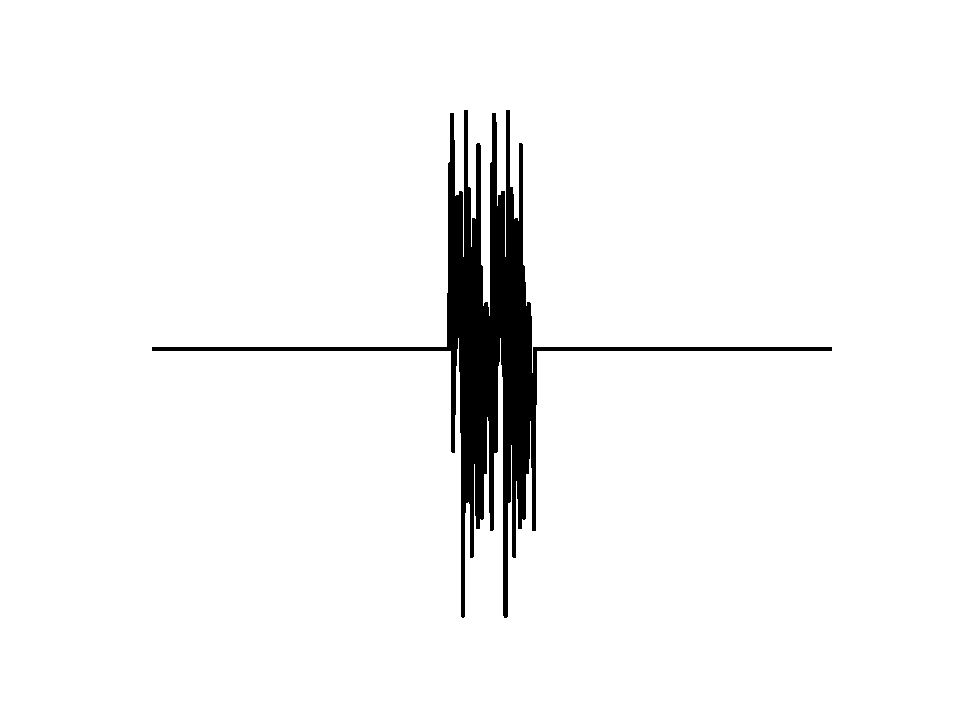
\includegraphics[width=1.5cm]{diagrams/xcorr_tagger_sync_padded.pdf}}
  }
  (sync_padded.north) node[anchor=south, align=center]{\small{Reference}\\\small{preamble}};

  % Precomupted box
  \draw[color=gray, densely dotted]
  (sync_padded.north west)
  ++(-0.25, 1) node[anchor=south west]{precomputed} coordinate(pbox_start)
  (ref_conj.south east)
  ++(0.25, -0.25) coordinate(pbox_end)
  (pbox_start) rectangle (pbox_end);


  \draw
  (ifft.north) to[short]
  ++(0, 0.8) node[anchor=south,inner sep=0](find_max) {
    \fbox{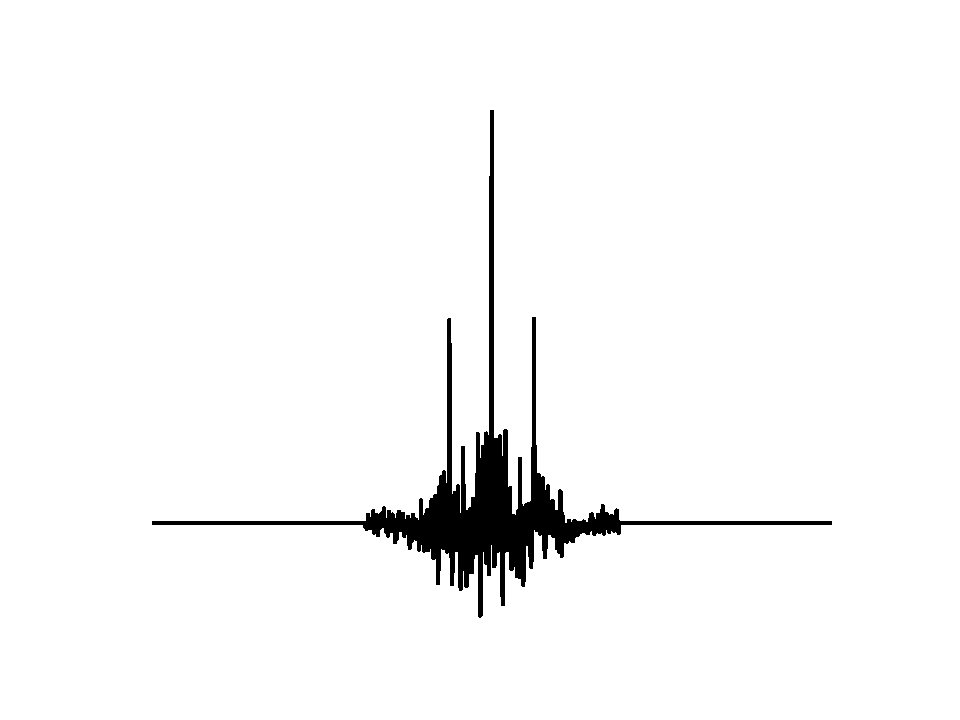
\includegraphics[width=1.5cm]{diagrams/xcorr_tagger_find_max.pdf}}
  }
  (find_max.north) to[short, -*]
  ++(0, 0.4) node[anchor=west, align=center]{\small{Mask using S\&C} information} to[short]
  ++(0, 0.4) node[anchor=south,inner sep=0](find_max_padded) {
    \fbox{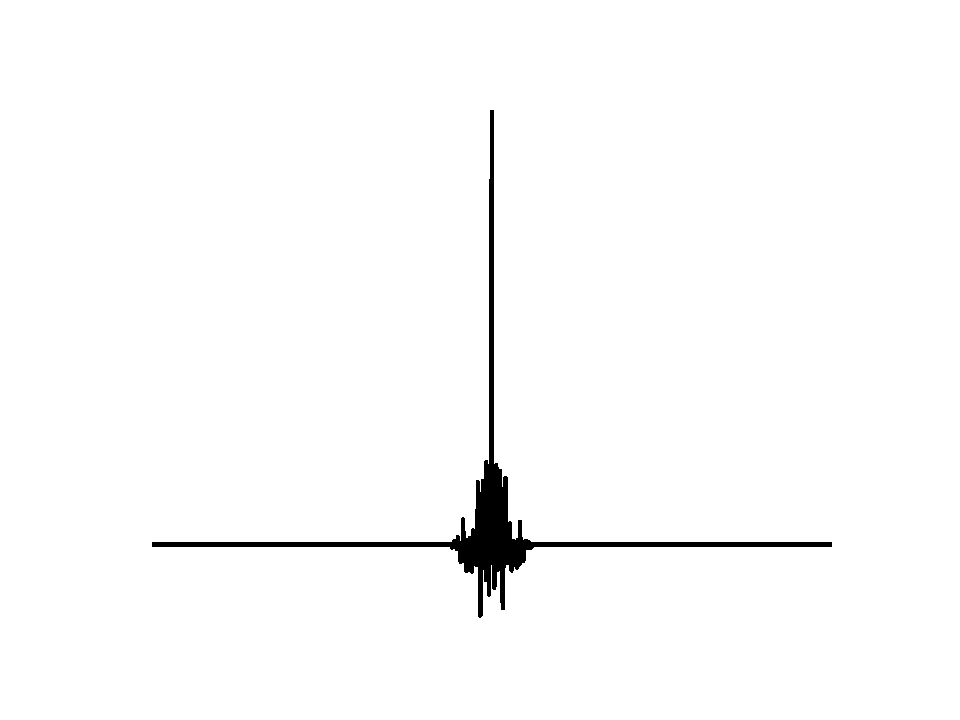
\includegraphics[width=1.5cm]{diagrams/xcorr_tagger_find_max_masked.pdf}}
  }
  (find_max_padded.north) to[short, -*]
  ++(0, 0.4) coordinate(find_split) to[short]
  (move_tag.south)
  (find_split) to[short]
  ++(-0.9, 0) node(thres)[minimum width=1.2cm, minimum height=1cm, anchor=east, draw=black, line width=0.25mm, align=center]{\small{Thres-}\\\small{hold}}
  (thres.west) to[short]
  ++(-0.5, 0) to[short]
  ++(0, 0.7) node[inputarrow, rotate=90]{};
\end{tikzpicture}
